%% Run LaTeX on this file several times to get Table of Contents,
%% cross-references, and citations.

\documentclass[12pt]{book}
\usepackage{Wiley-AuthoringTemplate}
\usepackage{chapterbib}
\usepackage[sectionbib,authoryear]{natbib}% for name-date citation comment the below line
%\usepackage[sectionbib,numbers]{natbib}% for numbered citation comment the above line
\usepackage{lettrine}

%%********************************************************************%%
%%       The below macro controls the numbering of section heads      %%
%% 0= no section numbers, 1= section, 2= subsection, 3= subsubsection %%
\setcounter{secnumdepth}{3}
%%********************************************************************%%

%%**********************************************************************%%
%%  The below macro controls the number of section heads displayed in   %%
%%			Table of Contents?				%%
%% 0= chapter, 1= section, 2= subsection, 3= subsubsection titles.	%%
\setcounter{tocdepth}{2}
%%**********************************************************************%%

%%\includeonly{fm}

\makeindex% for index generation

\begin{document}

\frontmatter
\documentclass[12pt]{osa-supplemental-document}
\setboolean{shortarticle}{false}

\title{Pengaruh Agen Bayaran dalam Pemilihan Pemimpin}
\author[1]{Winda Wijayasari - \texttt{20921003}}
\author[2]{Arizal Akbar Zikri - \texttt{20921008}}
\author[3]{Agus Hermawan - \texttt{20921302}}
\affil[1,2,3]{Sains Komputasi, FMIPA ITB}

\begin{abstract}
\end{abstract}

\setboolean{displaycopyright}{false} %copyright statement should not display in the  supplementary document

\mainmatter

\chapter{Pendahuluan}

\maketitle% This tag is required to print author and address in the output

\lettrine[loversize=1,lraise=0.3,lines=2]{A}{gen} merupakan individu atau objek yang memiliki ciri khas dan tindakan serta tujuan untuk melakukan suatu perhitungan tertentu secara otomatis dalam suatu lingkungan. Agent Based Modeling (ABM) merupakan suatu fenomena interaksi antar agen atau agen dengan lingkungan dalam suatu lingkungan yang dapat dibuatkan ke dalam model komputasi. Lingkungan merupakan suatu bentangan di mana agen-agen dapat berinteraksi, dipetakan, memiliki hubungan, dan digambarkan ke dalam bentuk data. Melalui pendekatan ABM, dapat memudahkan dalam melakukan eksplorasi, visualisasi dan analisis fenomena alam yang terjadi.

\section{This is First Level Heading}

\lipsum[1-2]

\subsection{This is Second Level Heading}

\lipsum[3]

For example, multiple citations from the \index{bibliography} of this \index{article}:
citet: \citet{CR7,CR8}, citep: \citep{CR9,CR6}.
As you see in Table~\ref{tab1-2}, the citations are \index{automatically!hyperlinked!citations} to their
reference in the bibliography. Refer Figure~\ref{fig1-1} for details:

\begin{figure}

\includegraphics{01.eps}
\caption{Figure Caption. Figure Caption.
Figure Caption. Figure Caption. Figure Caption. 
Figure Caption. Figure Caption.
\label{fig1-1}}
\end{figure}

For example, multiple citations from the \index{bibliography} of this \index{article}:
citet: \citet{CR9,CR6}, citep: \citep{CR9,CR6}.
As you see in Table~\ref{tab1-1}, the citations are \index{main entry with turn over lines main entry with turn over lines!subentry with turn over lines subentry with turn over lines!subsubentry with turn over lines subsubentry with turn over lines} to their
reference in the bibliography (Equation~\ref{eq1-1}).
\begin{equation}
\mathcal{L}\quad \mathbf{\mathcal{L}} = i \bar{\psi} \gamma^\mu D_\mu \psi - 
\frac{1}{4} F_{\mu\nu}^a F^{a\mu\nu} - m \bar{\psi} \psi\label{eq1-1}
\end{equation}

\subsubsection{This is Third Level Heading}

The manifestation of solar activity (flares, bursts, and others) occurs over the whole Sun, and most of radio astronomy observations are made from the Earth's surface, whereas a significant part of solar radio events (those from the far side of the Sun) is not available for terrestrial observers.
\begin{equation}
\mathcal{L}\quad \mathbf{\mathcal{L}} = i \bar{\psi} \gamma^\mu D_\mu \psi - 
\frac{1}{4} F_{\mu\nu}^a F^{a\mu\nu} - m \bar{\psi} \psi\label{eq1-2}
\end{equation}

\paragraph{This is Fourth Level Heading}

\lipsum[5]

\begin{table}
\caption{Enter table caption here.\label{tab1-1}}{%
\begin{tabular}{@{}cccc@{}}
\toprule
Tap     &Relative   &Relative   &Relative mean\\
number  &power (dB) &delay (ns) &power (dB)\\
\midrule
3 &0$-9.0$  &68,900\footnotemark[1] &$-12.8$\\
4 &$-10.0$ &12,900\footnotemark[2] &$-10.0$\\
5 &$-15.0$ &17,100 &$-25.2$\\
\botrule
\end{tabular}}{\footnotetext[]{Source: Example for table source text.}
\footnotetext[1]{Example for a first table footnote. Example for a first table footnote. Example for a first table footnote. Example for a first table footnote.}
\footnotetext[2]{Example for a second table footnote.}}
\end{table}

\subparagraph{This is Fifth Level Heading}

\lipsum[6]

The manifestation of solar activity (flares, bursts, and others) occurs over the whole Sun, and most of radio astronomy observations are made from the Earth's surface, whereas a significant part of solar radio events (those from the far side of the Sun) is not available for terrestrial observers (Equation~\ref{eq1-2}).

\begin{table}
\caption{Enter table caption here.\label{tab1-2}}{%
\begin{tabular}{@{}cccc@{}}
\toprule
Tap     &Relative   &Relative   &Relative mean\\
number  &power (dB) &delay (ns) &power (dB)\\
\midrule
3 &0$-9.0$  &68,900\footnotemark[1] &$-12.8$\\
4 &$-10.0$ &12,900\footnotemark[2] &$-10.0$\\
5 &$-15.0$ &17,100 &$-25.2$\\
\botrule
\end{tabular}}{\footnotetext[]{Source: Example for table source text.}
\footnotetext[1]{Example for a first table footnote. Example for a first table footnote. Example for a first table footnote. Example for a first table footnote.}
\footnotetext[2]{Example for a second table footnote.}}
\end{table}

\backmatter

\bibliographystyle{plainnat}
\bibliography{wiley}%


\section{Studi Pemilihan Pemimpin di ABM}

\lettrine[nindent=-0.01em,findent=0.2em]{M}{etode} ABM sangat ampuh digunakan dalam memodelkan permasalahan sehari-hari karena dapat memodelkan masalaah tanpa melibatkan banyak proses matematika yang rumit \cite{crooks2018agent}. Pemilihan pemim-pin menjadi salah satu contoh masalah yang dapat dimodelkan di ABM. Munculnya sistem pemerintahan yang demokrasi membawa semakin banyak pihak yang terlibat dalam proses pembuatan keputusan dan memperbanyak variabel dalam menghitung peluang para calon untuk dapat memenangkan pemilihan \cite{feddersen2004rational}, terutama perilaku setiap orang dan interaksi didalamnya sangat berpengaruh terhadap hasil dari pemilihan. Banyak penelitian dilakukan untuk masalah pemilihan (voting) ini \cite{feddersen2004rational,saaty1989group}. Dalam skala kecil, masalah voting bisa hanya permasalahan membagi sekelompok murid ke dalam dua tim yaitu  merah dan biru, tetapi dalam masalah yang lebih besar dapat dikaitkan pada pemilihan presiden atau pemilihan pemimpin serikat negara. Kasus pemilihan pemimpin ini dapat diselesaikan menggunakan ABM dimana para pelaku pemilih dipandang sebagai agen-agen yang berperan didalamnya. Background dari agen dan cara berinteraksi dapat dijadikan sebagai dasar  dari aturan interaksi dalam membangun model dari pemilihan \cite{kazil2020utilizing}.

Banyak hal yang mempengaruhi setiap individu dalam melakukan pemilihan atau bahkan memilih untuk tidak memilih. Dalam artikel \cite{olson2012logic} terdapat konsep rasionalitas instrumental, yang menurutnya individu rasional membuat pilihan yang mereka yakini akan membawa hasil yang paling mereka sukai, Olson berpendapat bahwa ada sedikit insentif rasional bagi individu untuk berkontribusi pada produksi barang publik (atau umum), mengingat mereka (para calon) yang mengeluarkan biaya, para pemilih akan tetap memperoleh benefit terlepas dari ikut berkontribusi (suara) atau tidak \cite{savigny_2014}. Pandangan ini meningkatkan jumlah pemilih yang memilih untuk tidak memilih (golput) pada acara pemilihan.

Pada tahun 2019, di Indonesia melakukan pemilihan umum baik legislative maupun presiden. Menurut tim Lembaga Survey Indonesia (LSI), mereka menyatakan bahwa jumlah golput untuk pemilihan presiden di tahun 2019 yaitu sekitar 19.24\% yang telah menurun dibandingkat Pilpresa sebelumnya di tahun 2014 yang mencapai 30.42\% \cite{bbc_2019}. Presentase tersebut sangatlah tinggi sehingga banyak usaha yang dilakukan untuk meningkatkan minat pemilih untuk ikut berpartisipasi melalui berbagai cara, baik itu melalui hadiah dan promo bagi yang telah melakukan kewajibannya untuk memilih hingga ancaman bila tidak berpartisipasi.

Melakukan pemilihan sebenarnya adalah reaksi rasional dari setiap individu \cite{feddersen2004rational}. Salah satu hal yang banyak dilakukan adalah dengan menempatkan aktor-aktor strategis yang dapat mengarahkan pemikiran secara rasional dari individu untuk melakukan pemilihan. Dalam pemilihan pendahuluan, ada bukti bahwa pemilih mengkondisikan pilihan suara mereka pada kelayakan kandidat \cite{abramson1992sophisticated}. Dalam sebuah studi komprehensif, penulis \cite{cox1997making} menunjukkan bahwa pola pemungutan suara dan hasil pemilu secara umum konsisten dengan pola perilaku yang diprediksikan oleh model voting strategis, misalnya di bawah aturan pluralitas (di mana kandidat dengan suara terbanyak memenangkan pemilihan).

Agen-agen strategis yang diterapkan pada penelitian ini adalah agen bayaran. Dalam hal ini, agen bayaran akan bertugas untuk mempengaruhi agen lain untuk mengikuti pilihan dari agen bayaran tersebut. Sehingga secara rasional para agen pemilih mengalami kenaikkan kecenderungan untuk mengikuti agen pemilih bayaran memilih pilihan. Model ini akan memperlihatkan bagaimana jumlah pemilih bayaran dapat berpengaruh dan bagaimana sekelompok kecil pemilih bayaran bila berada di posisi yang tepat akan mempercepat agen-agen pemilih untuk menentukan pilihannya.

Model pemilihan umum telah banyak diteliti baik di Indonesia maupun di dunia \cite{abramson1992sophisticated,cox1997making,wijayati2020money}. Untuk membangun model agen bayaran dalam pemilihan umum pemimpin, dimulai dengan model sederhana yaitu model voting yang terdapat pada NetLogo \cite{wilensky1999netlogo}, lalu model standing ovation yang dikembangkan oleh Miller dan Page \cite{miller2004standing}, dan seiring dengan meningkatnya komputasi untuk melakukan pemodelan, muncul MESA yang dikembangkan dengan bahasa Python \cite{kazil2020utilizing}. Model ini diharapkan dapat menggambarkan situasi pemilihan umum dengan banyak faktor yang mempengaruhi perilaku para pemilih. Salah satu yang akan ditekankan pada model ini adalah perilaku pemilih yang bergerak karena adanya aktor-aktor strategis yang menjadi gambaran seorang agen bayaran yang selanjutnya akan meningkatkan jumlah suara pemilih dan mempengaruhi hasil akhir dari pemilihan.

\subsection{Model Voting dari modul library NetLogo}

Untuk model pemilihan sebagai model paling sederhana dapat dilihat pada model voting yang disediakan oleh modul libraries Netlogo dan juga model standing ovation yang telah dikembangkan. Pada model voting, opini para agen akan terlihat dengan bagaimana setiap agen menentukan pilihannya berdasarkan observasi terhadap neighbours atau sekitarnya. Menurut penulis \cite{viridi2019agent} agen menempati satu sel grid yang lalu bergerak mengikuti pola yang ditetapkan.

Untuk memahami kestabilan suatu grup, model perlu diperbesar untuk mengurangi cluster dan  dan memahami konfigurasi saat dia stabil. Sebagai contoh, saat suatu sel dikelilingi (4 biru dan 4 hijau) disekitarnya maka posisi sel tersebut tidak akan berubah lagi. Meski demikian, hal ini tidak mudah bagi kita untuk memprediksi initial set dari suatu sel dan dimana batasnya hingga akhirnya kestabilan tercapai.

Sebagai gambaran, pemilih ditentukan di awal adalah jumlah pemilih warna hijau.

\begin{equation}
	InitialGreenVoter = CountPatches \times \frac{InitialGreen}{100}
\end{equation}

\texttt{InitialGreenVoter} dapat dikatakan merepresentasikan estimasi dari jumlah keberpihakan suatu kelompok di lingkungan dan jumlah tick menggambarkan waktu yang menunjukkan bagaimana perkembangan keberpihakan dari setiap patch menurut waktu seperti Gambar \ref{fig:initvoter} berikut.

\begin{figure}[H]
	\centering
	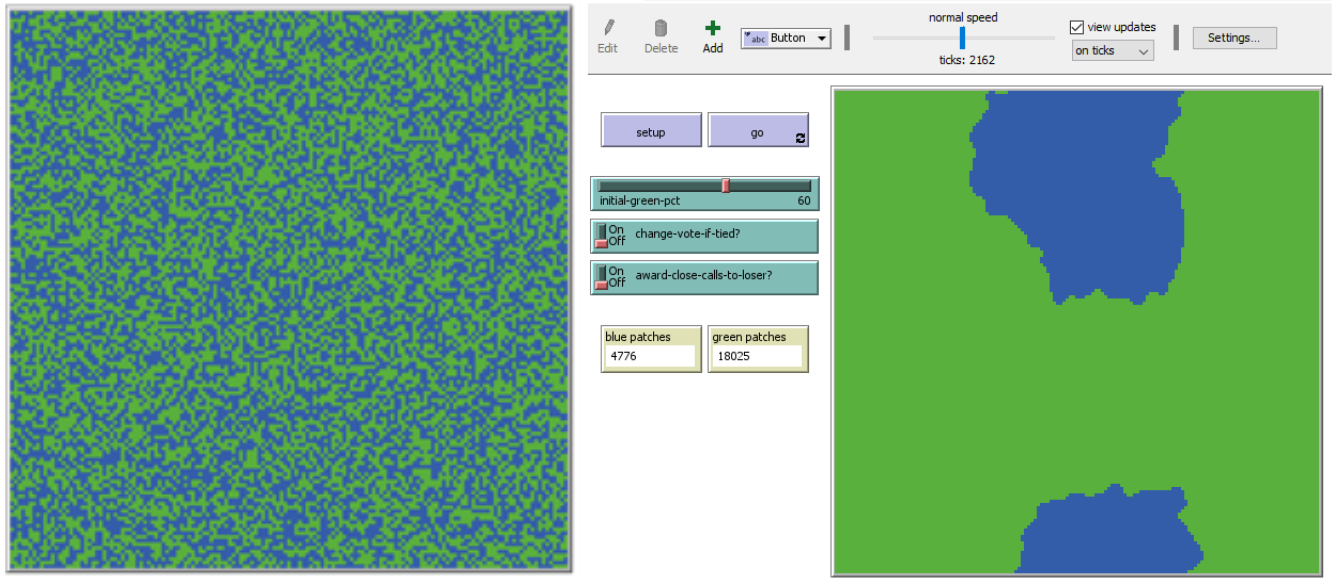
\includegraphics[width=\linewidth]{images/ch03/InitVoter}
	\caption{Simulasi voting NetLogo}
	\label{fig:initvoter}
\end{figure}

\subsubsection{Aturan sederhana pada model voting}

Pada model ini terdapat basic rules diantaranya sebagai berikut:

\begin{itemize}
	\item Bila neighbours menunjukkan jumlah opini seri, maka sel akan tetap pada pilihan terakhir dan tidak berubah lagi seterusnya

	\item Agen akan selalu mengikuti pilihan dari mayoritas dari agen-agen disekitarnya
\end{itemize}

Pada model awal, jumlah initial patch green menentukan, artinya bila suatu kelompok sudah memiliki kecenderungan, kemungkinan komunitas akan mengikuti. Pada gambar di bawah, proporsi hijau diatur 50\% di awal, berkat ada interaksi antar agen jumlah akhir pemenangnya adalah biru dengan selisih yang tidak terlalu besar.

\begin{figure}[H]
	\centering
	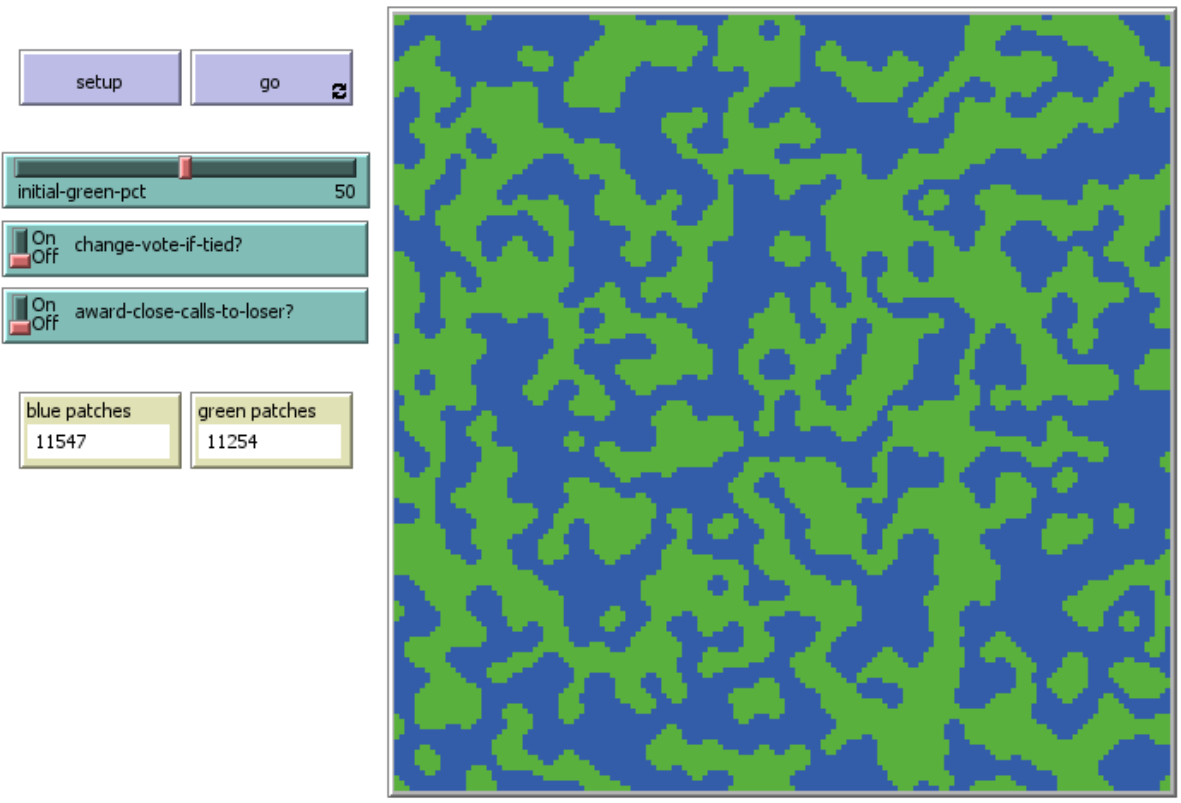
\includegraphics[width=\linewidth]{images/ch03/Voter2}
	\caption{Interaksi antar agen pemilih}
	\label{fig:voter2}
\end{figure}

\subsubsection{Modifikasi model}

\textbf{Change vote if tied}. Aturan default dari model ini adalah bila neighbours menunjukkan jumlah opini seri, maka sel akan tetap pada pilihan terakhir dan tidak berubah lagi seterusnya.

Opsi ini dapat merubah rule: bila seri, maka sel akan berubah. Hal ini membuat ketidakstabilan  dalam system yang menghasilkan noisy pada kesetimbangan. Hasilnya para agen tidak akan pernah berhenti bahkan saat sudah mencapai kestabilan global. Meski demikian, secara umum opsi ini tidak akan merubah skor dari distribusi opini, tetapi akan mengakibatkan beberapa agen merubah opini mereka secara terus menurus pada konfigurasi ini. Hasil simulasi pada modifikasi ini dapat dilihat dalam Gambar \ref{fig:voter3}.

\begin{figure}[H]
	\centering
	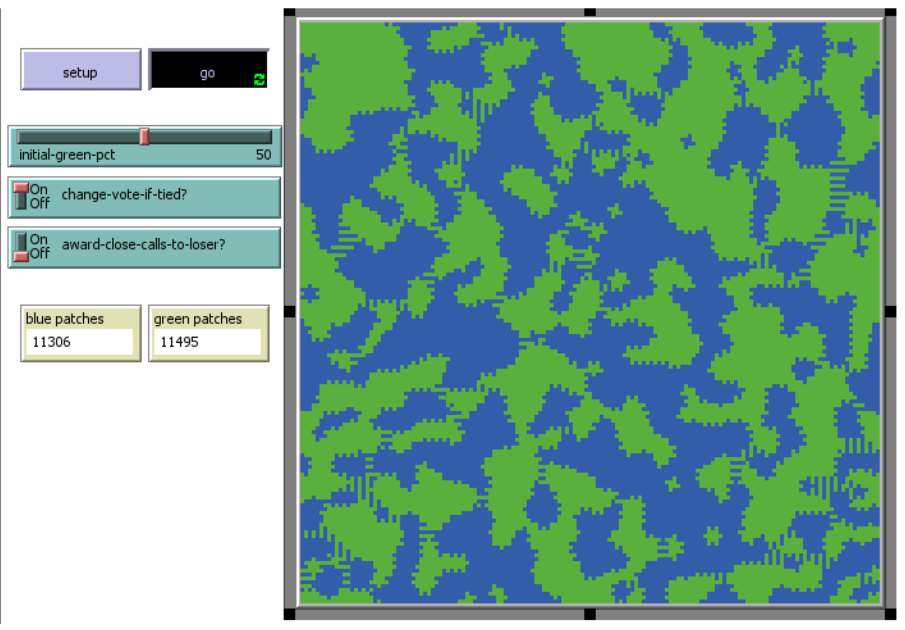
\includegraphics[width=\linewidth]{images/ch03/Voter3}
	\caption{Perubahan konfigurasi untuk pemilihan seri}
	\label{fig:voter3}
\end{figure}

\textbf{Award close calls to loser}. Konfigurasi dasar model ini adalah agen akan selalu mengikuti pilihan dari mayoritas dari agen-agen disekitarnya. Opsi ini meminta agen untuk memilih posisi minoritas secara sistemik. Dengan ini, hasil dari pemilihan bisa diluar ekspektasi. Dapat dibayangkan suatu society yang dipenuhi oleh agen-agen kontradiktif yang secara constant selalu berusaha merubah hasil. Lalu saat kesetimbangan sulit tercapai, dan minority tidak dapat mengubah pilihannya, system akan terus-menerus berubah menjadi satu warna dengan beberapa gelembung minoritas yang kecil didalamnya lalu menghadirkan ketidakstabilan yang tinggi.

Namun, untuk memperoleh hasil konstan seperti ini memerlukan waktu yang cukup lama. Kedua jenis agen ini dapat hidup bersama dalam jangka waktu yang cukup lama. Terkadang kelas yang kalah kembali menyamakan kedudukan dengan yang menang, terkadang dia terus berisolaso antara 8000-9000 melawan mayoritas 13000-12000.

Hal yang dapat dipahami dari Gambar \ref{fig:voter4} adalah bahwa dalam komunitas masyarakat demokrasi, hasil pemungutan suara pada saat-saat tertentu dapat berubah dan tidak terduga dan tidak dapat dikatakan menjadi dasar sebagai perkiraan hasil pada pemungutan suara yang lain.

\begin{figure}[H]
	\centering
	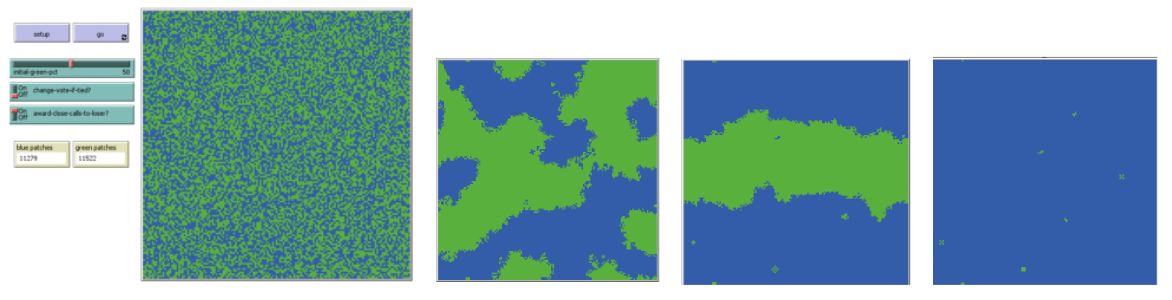
\includegraphics[width=\linewidth]{images/ch03/Voter4}
	\caption{Perubahan bertahap selama voting}
	\label{fig:voter4}
\end{figure}

Setelah 90.000 iterasi model masih belum mencapai titik kesetimbangan. Walaupun dapat diramalkan bahwa model akan berakhir dimenangkan oleh patch biru dan terdapat beberapa titik-titik hijau.

Pada konsep pemilihan umum dengan pemilih bayaran yang akan dikembangkan, para agen netral akan digiring oleh agen-agen bayaran yang ditempatkan untuk membuat pilihan mengikuti pilihan dari agen bayaran. Bagaimana perilaku dari agen dapat terpengaruh oleh agen lain, dapat dilihat pada bagian model standing ovation berikut.

\subsection{Model Standing Ovation}

Model standing ovation pertama kali dikenalkan oleh Miller dan Page (2004) dengan mengilustrasikan masalah pengambilan keputusan, yaitu bagaimana para penonton pada akhirnya akan ikut berdiri dan bertepuk tangan. Pada situasi tersebut, setiap penonton perlu memutuskan apa dia akan ikut berdiri atau tetap duduk diam. Tetapi, hal tersebut akan berubah bilamana dia dikekelingi oleh orang-orang yang berdiri dan bertepuk tangan. Hal ini terjadi secara alami untuk menghindari perasaan tidak nyaman karena berbeda dengan orang lain. Sama halnya dengan tidak mungkin seseorang merasa nyaman berdiri dan bertepuk tangan di saat semua orang duduk terdiam.

Pada model Miller dan Page, Terdapat sebuah auditorium berukuran $L \times L$ yang sesak dipenuhi oleh agen. Di akhir pertunjukkan, penonton akan mengevaluasi pertunjukkan berdasarkan dari jumlah tepuk tangan. Nilai persepsi dari agen $i$ merupakan nilai floating poin acak $\left( 0.1 \right) $ yang disebut $qi$ dan model ini ditentukan nilai batas sebesar $\left( 0.5 \right)$ apabila $qi > 0.5$.

Pada langkah selanjutnya, agen akan meninjau sekelilingnya jika sekelilingnya menunjukkan perilaku yang berbeda maka agen dapat merubah keputusannya. Model Miller dan page membuat dua jenis environment yaitu lima tetangga dan kerucut.

\begin{itemize}
	\item Pada skenario lima tetangga, agen akan memperhatikan agen yang berada di samping kanan, kiri, depan, dan belakang seperti Table \ref{tbl:formasi_sop}.

	\begin{table}[H]
		\centering
		\begin{tabular}{|c|c|c|}
			\hline
			F & \cellcolor{gray!30}F & F \\
			\hline
			\cellcolor{gray!30}F & \cellcolor{gray!50}X & \cellcolor{gray!30}F \\
			\hline
			F & \cellcolor{gray!30}F & F \\
			\hline
		\end{tabular}
		\caption{Formasi lima tetangga}
		\label{tbl:formasi_sop}
	\end{table}

	\item Pada skenario kerucut, agen akan melihat agen lain di sisi kanan dan kirinya, lalu tiga agen di baris pertama depan dan lima agen di baris kedua depan dan seterusnya seperti Tabel \ref{tbl:formasi_kerucut}.

	\begin{table}[H]
		\centering
		\begin{tabular}{|c|c|c|c|c|c|c|}
			\hline
			\cellcolor{gray!30}F & \cellcolor{gray!30}F & \cellcolor{gray!30}F & \cellcolor{gray!30}F & \cellcolor{gray!30}F & \cellcolor{gray!30}F & \cellcolor{gray!30}F \\
			\hline
			F & \cellcolor{gray!30}F & \cellcolor{gray!30}F & \cellcolor{gray!30}F & \cellcolor{gray!30}F & \cellcolor{gray!30}F & F \\
			\hline
			F & F & \cellcolor{gray!30}F & \cellcolor{gray!30}F & \cellcolor{gray!30}F & F & F \\
			\hline
			F & F & \cellcolor{gray!30}F & \cellcolor{gray!50}X & \cellcolor{gray!30}F & F & F \\
			\hline
		\end{tabular}
		\caption{Formasi kerucut}
		\label{tbl:formasi_kerucut}
	\end{table}
\end{itemize}

\subsubsection{Aturan pada model standing ovation}
Ada aturan yang diterapkan di model standing ovation, yaitu:
\begin{enumerate}
	\item \textbf{Synchronous updating} (SU) :Semua agen memperbaharui statusnya secara bersamaan di waktu yang sama.

	\item \textbf{Asyncronous-random updating} (ARU): Pada setiap waktu setiap agen mereview mereka dengan urutan random
\end{enumerate}

\subsubsection{Penerapan model standing ovation di NetLogo}

Pada model lima tetangga dapat dilakukan dengan  menggunakan model kerucut dengan panjang barisan 1. Pada kasus selanjutnya misalkan untuk $L=20$ (terdapat 20 baris penonton), maka model kerucut dapat diimplementasikan hingga $n=18$.


\begin{itemize}
	\item Skenario 1 – lima tetangga - synchronous updating

	Lima tetangga dengan nilai $cone-length=1$, $noise=0$, $intrinsic-proc-standing=0.42$, $updating=synchronous updating$ dan pengaturan yang dipilih \texttt{Make guy stand up}. Berikut akan diperlihatkan apa yang dilihat oleh agen.

	\begin{figure}[H]
		\centering
		\subfloat[Kondisi awal]{
			\label{sfig:sop1}
			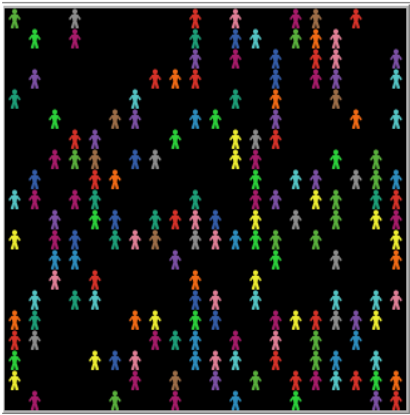
\includegraphics[width=0.3\linewidth]{images/ch03/sop1}
		}\hfill
		\subfloat[Saat $t=1$]{
			\label{sfig:sop2}
			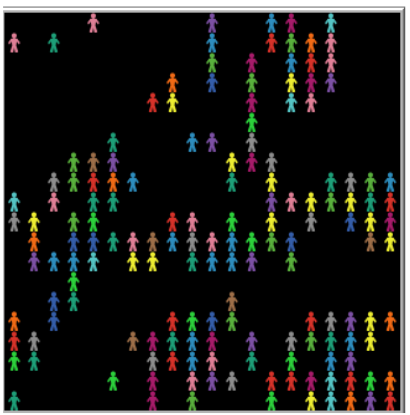
\includegraphics[width=0.3\linewidth]{images/ch03/sop2}
		}\hfill
		\subfloat[Saat $t=10$]{
			\label{sfig:sop3}
			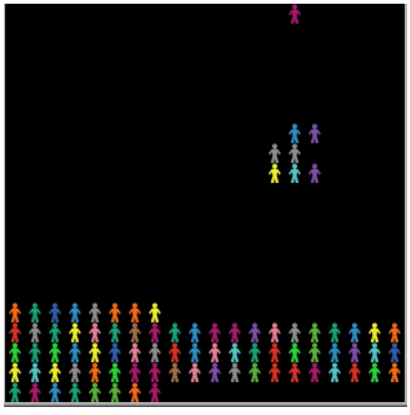
\includegraphics[width=0.3\linewidth]{images/ch03/sop3}
		}\hfill
		\caption{Proses iterasi standing ovation di NetLogo}
		\label{fig:proses_sop}
	\end{figure}

	Pada saat $t=27$ diperoleh dengan tidak ada seorangpun yang berdiri dengan $t$ menyatakan jumlah iterasi. Pada model ini, setiap agen bergerak mengikuti perubahan yang terjadi di sekitarnya.

	\begin{figure}[H]
	\centering
	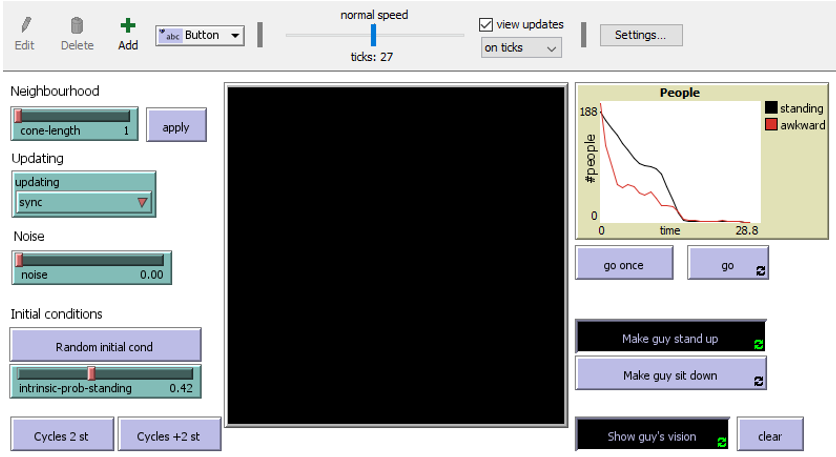
\includegraphics[width=\linewidth]{images/ch03/sop4}
	\caption{Hasil simulasi saat $t=27$}
	\label{fig:sop4}
	\end{figure}

	\item Skenario 1 – lima tetangga - asynchronous updating

	Lima tetangga dengan nilai $cone-length=1$, $noise=0$, $intrinsic-proc-standing=0.42$, $updating=asynchronous updating$ dan pengaturan yang dipilih \texttt{Make guy stand up}. Berikut akan diperlihatkan apa yang dilihat oleh agen.

	\begin{figure}[H]
		\centering
		\subfloat[Kondisi awal]{
			\label{sfig:sop4}
			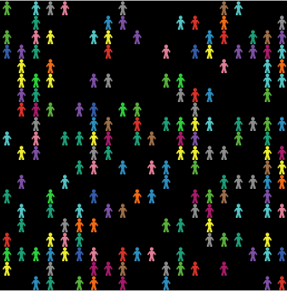
\includegraphics[width=0.3\linewidth]{images/ch03/sop5}
		}\hfill
		\subfloat[Saat $t=1$]{
			\label{sfig:sop5}
			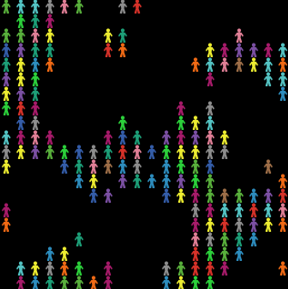
\includegraphics[width=0.3\linewidth]{images/ch03/sop6}
		}\hfill
		\subfloat[Saat $t=10$]{
			\label{sfig:sop6}
			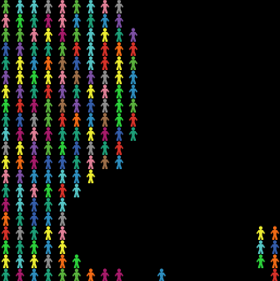
\includegraphics[width=0.3\linewidth]{images/ch03/sop7}
		}\hfill
		\caption{Proses iterasi standing ovation asynchronous updating di NetLogo}
		\label{fig:proses_sop_async}
	\end{figure}

	Pada skenario ini di iterasi $t=36$ agen masih belum konvergen dikarenakan agen secara random memperhatikan sekitarnya. Bisa dikatakan pada situasi ini seolah penonton terbagi di dua kelompok.

	\begin{figure}[H]
	\centering
	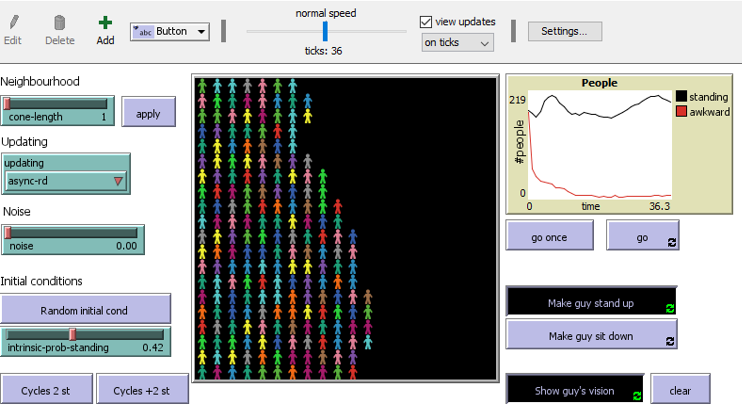
\includegraphics[width=\linewidth]{images/ch03/sop8}
	\caption{Hasil simulasi saat $t=36$}
	\label{fig:sop8}
	\end{figure}

	\item Skenario 2- Lingkungan kerucut - synchronous updating

	Kerucut dengan nilai $cone-length=18$, $noise=0.5$, $intrinsic-proc-standing=0.5$, $updating= synchronous updating$ dan pengaturan yang dipilih \texttt{Make guy stand up}. Berikut akan diperlihatkan apa yang dilihat oleh agen.

	\begin{figure}[H]
		\centering
		\subfloat[Kondisi awal]{
			\label{sfig:sop7}
			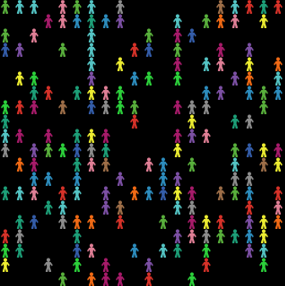
\includegraphics[width=0.3\linewidth]{images/ch03/sop9}
		}\hfill
		\subfloat[Saat $t=1$]{
			\label{sfig:sop8}
			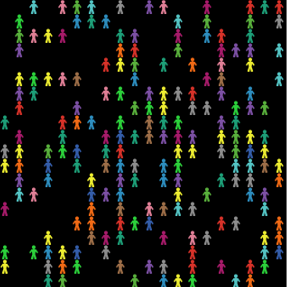
\includegraphics[width=0.3\linewidth]{images/ch03/sop10}
		}\hfill
		\subfloat[Saat $t=10$]{
			\label{sfig:sop9}
			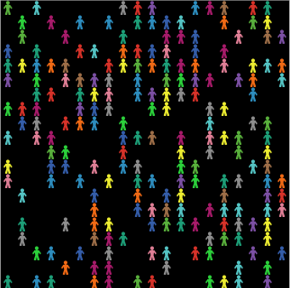
\includegraphics[width=0.3\linewidth]{images/ch03/sop11}
		}\hfill
		\caption{Proses iterasi standing ovation kerucut synchronous updating di NetLogo}
		\label{fig:proses_sop_kerucut_sync}
	\end{figure}

	Pada skenario ini, di iterasi $t=36$ agen masih belum konvergen dikarenakan pada kerucut jumlah pengaruh yang diterima setiap agen lebih tinggi. Pada perubahan setiap agen pada tiap waktu secara bersamaan, perubahan akan lebih mudah terprediksi karena sangat bergantung terhadap kondisi awal. Pada skenario 2, noise diaktifkan untuk memberikan perubahan dinamik pada model lebih signifikan. Noise juga membantu agar sistem tidak terkunci pada suatu state.

	\begin{figure}[H]
	\centering
	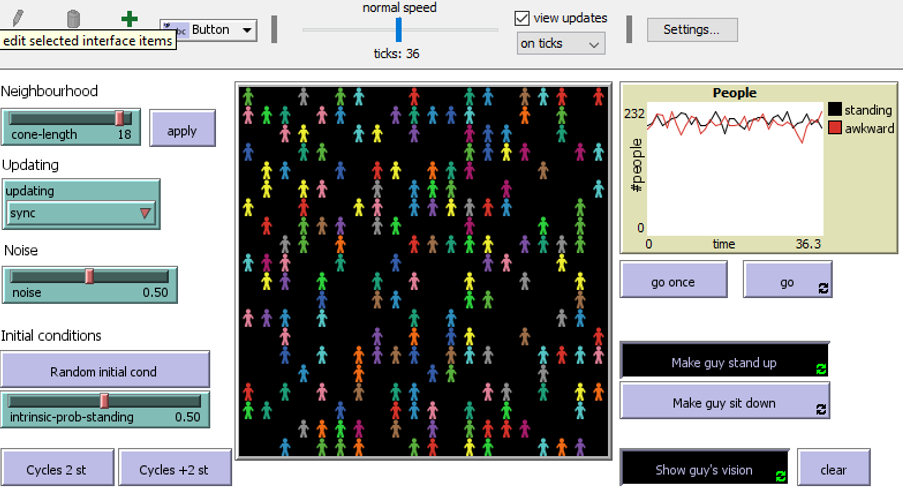
\includegraphics[width=\linewidth]{images/ch03/sop12}
	\caption{Hasil simulasi saat $t=36$}
	\label{fig:sop12}
	\end{figure}

	\item Skenario 2- Lingkungan kerucut - asynchronous updating

	Kerucut dengan nilai $cone-length=18$, $noise=0.5$, $intrinsic-proc-standing=0.5$, $updating=synchronous updating$ dan pengaturan yang dipilih \texttt{Make guy stand up}. Berikut akan diperlihatkan apa yang dilihat oleh agen.

	\begin{figure}[H]
		\centering
		\subfloat[Kondisi awal]{
			\label{sfig:sop10}
			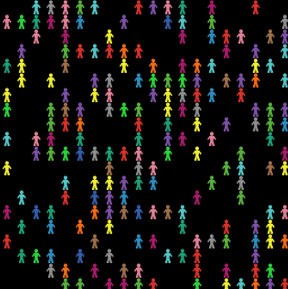
\includegraphics[width=0.3\linewidth]{images/ch03/sop13}
		}\hfill
		\subfloat[Saat $t=1$]{
			\label{sfig:sop11}
			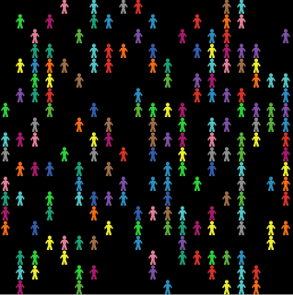
\includegraphics[width=0.3\linewidth]{images/ch03/sop14}
		}\hfill
		\subfloat[Saat $t=10$]{
			\label{sfig:sop12}
			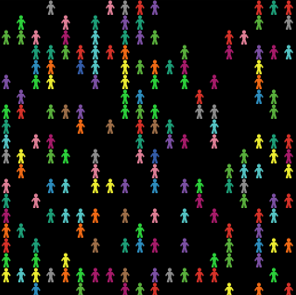
\includegraphics[width=0.3\linewidth]{images/ch03/sop15}
		}\hfill
		\caption{Proses iterasi standing ovation kerucut asynchronous updating di NetLogo}
		\label{fig:proses_sop_kerucut_async}
	\end{figure}

	Pada skenario ini, di iterasi $t=36$ agen masih belum konvergen dikarenakan pada kerucut jumlah pengaruh yang diterima setiap agen lebih tinggi. Karena setiap agen berubah secara random pada waktu yang berbeda. Maka, terdapat keterkaitan yang lebih rumit. Perubahan pada agen di baris $n+1$ tergantung pada perubahan agen di baris $n$.

	\begin{figure}[H]
	\centering
	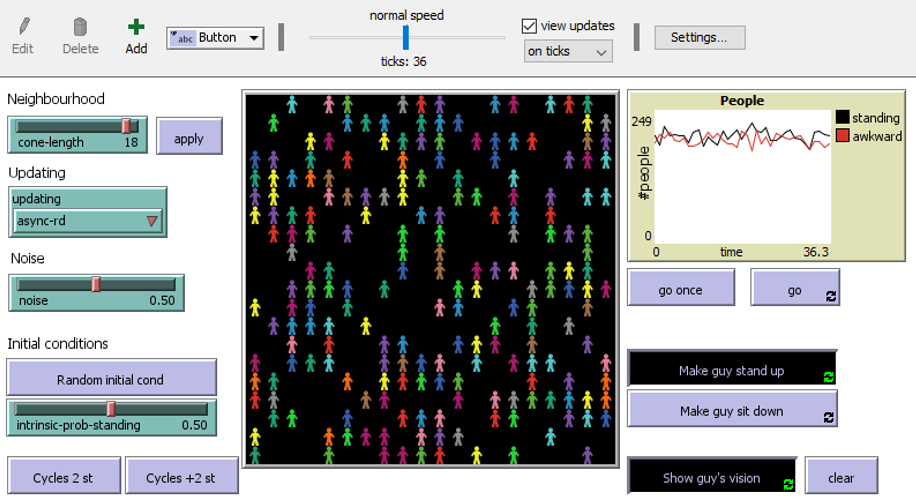
\includegraphics[width=\linewidth]{images/ch03/sop16}
	\caption{Hasil simulasi saat $t=36$}
	\label{fig:sop13}
	\end{figure}
\end{itemize}

Dalam kaitannya dengan pemilih bayaran, model standing ovation dapat dijadikan rujukan untuk menunjukkan bahwa individu dapat merubah keputusannya akibat ada perubahan di sekelilingnya dan noises memberikan state lebih dinamis.


\chapter{This is Chapter Three Title}

After reading this chapter you should be able to:

\begin{objectives}
\item List the main subsectors and components of the environmental and energy infrastructure

\item Explain \url{www.google.com} the function of each infrastructure sector

\item Identify components related to environmental and energy infrastructure
\end{objectives}

\section{This is First Level Heading}

\lipsum[1]

The manifestation of solar activity\footnote{This is an example for first text footnote. This is an example for first text footnote. This is an example for first text footnote.} (flares, bursts, and others) occurs over the whole Sun, and most of radio astronomy observations are made from the Earth's surface, whereas a significant part of solar radio events (those from the far side of the Sun) is not available for terrestrial observers.

\subsubsection*{Example for Quotes}

\begin{quote}[quote]

\title{Quote Head}

Quote Text  Quote Text  Quote Text  Quote Text Quote Text Quote Text 
Quote Text  Quote Text  Quote Text  Quote Text Quote Text Quote Text 

\source{Quote Source}

Quote Text  Quote Text  Quote Text  Quote Text Quote Text Quote Text 
Quote Text  Quote Text  Quote Text  Quote Text Quote Text Quote Text 

\source{Quote Source}

\end{quote}

\begin{quote}[quote]

``Quote Text  Quote Text  Quote Text  Quote Text Quote Text Quote Text 
Quote Text  Quote Text  Quote Text  Quote Text Quote Text Quote''
\source{Quote Source}

\end{quote}

\subsubsection*{Example for Extracts}

\begin{quote}[extract]
\title{Extract Head}
Extract Text  Extract Text  Extract Text  Extract Text Extract Text Extract Text 
Extract Text  Extract Text  Extract Text  Extract Text Extract Text Extract Text 
\source{Extract Source}

Extract Text  Extract Text  Extract Text  Extract Text Extract Text Extract Text 
Extract Text  Extract Text  Extract Text  Extract Text Extract Text Extract Text 
\source{Extract Source}
\end{quote}

\begin{quote}[extract]
``Extract Text  Extract Text  Extract Text  Extract Text Extract Text Extract Text 
Extract Text  Extract Text  Extract Text  Extract Text Extract Text Extract''
\source{Extract Source}
\end{quote}

\subsubsection*{Example for Pull quotes}

\begin{quote}[pullquote]

``Pull Quote Text  Pull Quote Text  Quote Text  Quote Text Quote Text Quote Text 
Quote Text  Quote Text  Quote Text  Quote Text Quote Text Quote''
\source{Pull Quote Source}

\end{quote}

\begin{quote}[pullquote]

Pull Quote Text  Quote Text  Quote Text  Quote Text Quote Text Quote Text 
Quote Text  Quote Text  Quote Text  Quote Text Quote Text Quote Text 

\source{Pull Quote Source}

Pull Quote Text  Quote Text  Quote Text  Quote Text Quote Text Quote Text 
Quote Text  Quote Text  Quote Text  Quote Text Quote Text Quote Text 

\source{Pull Quote Source}
\end{quote}

\subsubsection*{Example for Verse/Poetry}

\begin{quote}[poetry]

\title{Poetry Title}

Verse Text here Verse Text here Verse Text here Verse Text here

Verse Text here Verse Text here Verse Text here Verse Text hereVerse Text here Verse Text here Verse Text here Verse Text here

Verse Text here Verse Text here Verse Text here Verse Text here

Verse Text here Verse Text here Verse Text here Verse Text here

\source{Source: Verse/Poetry Source}
\end{quote}

\subsubsection*{Example for Epigraph}

\begin{quote}[epigraph]
Epigraph  without section head Text  Epigraph  Text  Epigraph  Text  
Epigraph  Text Epigraph  Text Epigraph  Text Epigraph  Text  Epigraph  
Text  Epigraph  Text 
\source{Epigraph Source}
\end{quote}

\subsubsection*{Example for Dialogue}

\begin{dialogue}

\item[Speaker A:] Dialogue Text. Dialogue Text. Dialogue Text. Dialogue Text. Dialogue Text. Dialogue Text. Dialogue Text. Dialogue Text. 

\item[Speaker B:] Dialogue Text. Dialogue Text. Dialogue Text. Dialogue Text. Dialogue Text. Dialogue Text. Dialogue Text. Dialogue Text.

\item[Speaker A:] Dialogue Text. Dialogue Text. Dialogue Text. Dialogue Text. Dialogue Text. Dialogue Text. Dialogue Text. Dialogue Text.

\end{dialogue}

\noindent
The manifestation of solar activity\footnote{This is an example for first text footnote. This is an example for first text footnote. This is an example for first text footnote.} (flares, bursts, and others) occurs over the whole Sun, and most of radio astronomy observations are made from the Earth's surface, whereas a significant part of solar radio events (those from the far side of the Sun) is not available for terrestrial observers.

\begin{exercises}[Exercises]

\item \label{3a} Item 1 What is the meaning of life?

\answer{Ans: b}

\begin{exercise}
\item for italic text
\item for bold text 
\item for small caps
\item for text with 
\end{exercise}

\item Item 2 What is the meaning of life?

\hint{Answering this requires Deep Thought.}

\answer{Ans: 42}

\explanation{See THHGTTG.}

\item Item 3 What is the meaning of life?

\end{exercises}

\noindent Another type of layout for exercises:

\begin{exer}
Exercise content. Exercise content. Exercise content. Exercise content. Exercise content. Exercise content. Exercise content. Exercise content. Exercise content. Exercise content.  Exercise content. Exercise content. Exercise content. Exercise content. Exercise content. Exercise content. Exercise content. Exercise content. Exercise content. Exercise content. Exercise content. Exercise content. Exercise content. Exercise content. Exercise content. Exercise content. Exercise content. Exercise content. Exercise content.

\solution{\textbf{Solution:} Solution Text. Solution Text. Solution Text. Solution Text. Solution Text. Solution Text. Solution Text. Solution Text. Solution Text. Solution Text. Solution Text. Solution Text. Solution Text. Solution Text. Solution Text. Solution Text. Solution Text. Solution Text. Solution Text.}
\end{exer}

\begin{exer}
Exercise content. Exercise content. Exercise content. Exercise content. Exercise content. Exercise content. Exercise content. Exercise content. Exercise content. Exercise content.  Exercise content. Exercise content. Exercise content. Exercise content. Exercise content. Exercise content. Exercise content. Exercise content. Exercise content. Exercise content. Exercise content. Exercise content. Exercise content. Exercise content. Exercise content. Exercise content. Exercise content. Exercise content. Exercise content.

\solution{\textbf{Solution:} Solution Text. Solution Text. Solution Text. Solution Text. Solution Text. Solution Text. Solution Text. Solution Text. Solution Text. Solution Text. Solution Text. Solution Text. Solution Text. Solution Text. Solution Text. Solution Text. Solution Text. Solution Text. Solution Text.}
\end{exer}

\chapter{This is Chapter Four Title}

After reading this chapter you should be able to:

\begin{objectives}
\item List the main subsectors and components of the environmental and energy infrastructure

\item Explain \url{www.google.com} the function of each infrastructure sector

\item Identify components related to environmental and energy infrastructure
\end{objectives}

\section{This is First Level Heading}

\lipsum[1-2]

The manifestation of solar activity\footnote{This is an example for first text footnote. This is an example for first text footnote. This is an example for first text footnote.} (flares, bursts, and others) occurs over the whole Sun, and most of radio astronomy observations are made from the Earth's surface, whereas a significant part of solar radio events (those from the far side of the Sun) is not available for terrestrial observers.

\subsubsection*{Example for Feature Fixed}

\begin{featureFixed}[tip]

\title{TIP Feature Head}Featurefixed Text Featurefixed Text Featurefixed Text Text
Featurefixed Text Featurefixed Text Featurefixed Text Featurefixed Text
Featurefixed Text Featurefixed Text Featurefixed Text Featurefixed Text
Featurefixed Text Featurefixed Text Featurefixed Text Featurefixed Text
Featurefixed Text Featurefixed Text Featurefixed Text Featurefixed Text
Featurefixed Text Featurefixed Text Featurefixed Text Featurefixed Text.

\end{featureFixed}

\begin{featureFixed}[]

\title{FEATURE FIXED HEAD}Feature Fixed Feature Featurefixed Text Featurefixed Text Featurefixed Text
Featurefixed Text Featurefixed Text Featurefixed Text Featurefixed Text
Featurefixed Text Featurefixed Text Featurefixed Text Featurefixed Text
Featurefixed Text Featurefixed Text Featurefixed Text Featurefixed Text.
\end{featureFixed}

\subsubsection*{Example for Boxes}

The sample for unnumbered Figure with caption

\begin{unnumfigure}

\includegraphics[scale=0.5]{01.eps}
\caption{\title{Unnumbered Figure Title}Unnumbered Figure caption. Unnumbered Figure caption. Unnumbered Figure caption. Unnumbered Figure caption.
\source{Unnumbered Figure Source}}
\end{unnumfigure}

\clearpage

The sample for unnumbered Figure without caption

\begin{unnumfigure}

\includegraphics{01.eps}
\end{unnumfigure}

\begin{sidewaysfigure}

\includegraphics{01.eps}
\caption{\title{Figure Title}Figure Caption. Figure Caption.
Figure Caption. Figure Caption. Figure Caption.
Figure Caption. Figure Caption. \source{\textit{Source:} Figure Source.}
\label{fig4-2}}
\end{sidewaysfigure}

\clearpage

\begin{sidewaystable}[tbh]
\def\arraystretch{1.2}
\caption{Enter sideways table caption here.\label{tab1}}{%
\begin{tabular}{@{}cccc@{}}
\toprule
Tap &Relative &Relative &Relative mean\\
number  &power (dB) &delay (ns) &power (dB)\\
\midrule
3 & 0$-9.0$ & 68,900 & $-12.8$\\
4 & $-10.0$ & 12,900 & $-10.0$\\
5 & $-15.0$ & 17,100\footnotemark[1] & $-25.2$\\
\botrule
\end{tabular}}{\footnotetext[1]{This is table footnote}}
\end{sidewaystable}

This is an unnumbered table

\begin{unnumtable}
\caption{Enter unnumbered table caption here. Enter unnumbered table caption here. Enter unnumbered table caption here.}{%
\begin{tabular}{@{}cccc@{}}
\toprule
Tap &Relative &Relative &Relative mean\\
number  &power (dB) &delay (ns) &power (dB)\\
\midrule
3 & 0$-9.0$ & 68,900 & $-12.8$\\
4 & $-10.0$ & 12,900 & $-10.0$\\
5 & $-15.0$ & 17,100 & $-25.2$\\
6 & $-20.0$ & 20,000\footnotemark[1] & $-16.0$\\
\botrule
\end{tabular}}{\footnotetext[1]{This is unnumbered table footnote}
\footnotetext[]{Source: This is unnumbered table source. This is unnumbered table footnote}}
\end{unnumtable}

\clearpage

For Unnumbered Table without caption and source/note:

\begin{unnumtable}
\caption{}{%
\begin{tabular}{@{}cccc@{}}
\toprule
Tap &Relative &Relative &Relative mean\\\noalign{\vskip-6pt}
number  &power (dB) &delay (ns) &power (dB)\\
\midrule
3 & 0$-9.0$ & 68,900 & $-12.8$\\
4 & $-10.0$ & 12,900 & $-10.0$\\
5 & $-15.0$ & 17,100 & $-25.2$\\
6 & $-20.0$ & 20,000 & $-16.0$\\
\botrule
\end{tabular}}{}
\end{unnumtable}




\chapter{This is Chapter Five Title}

After reading this chapter you should be able to:

\begin{objectives}
\item List the main subsectors and components of the environmental and energy infrastructure

\item Explain \url{www.google.com} the function of each infrastructure sector

\item Identify components related to environmental and energy infrastructure
\end{objectives}

\section{This is First Level Heading}

\lipsum[1-2]

The manifestation of solar activity\footnote{This is an example for first text footnote. This is an example for first text footnote. This is an example for first text footnote.} (flares, bursts, and others) occurs over the whole Sun, and most of radio astronomy observations are made from the Earth's surface, whereas a significant part of solar radio events (those from the far side of the Sun) is not available for terrestrial observers.

\subsubsection*{Enunciations}
 
For bold head and italic body:

\begin{theorem}[Theorem Title]
Theorem content. Theorem content. Theorem content. Theorem content. Theorem content. 
\end{theorem}

\begin{lemma}
Lemma content. Lemma content. Lemma content. Lemma content. Lemma content. Lemma content. 
Lemma content. 
Lemma content. 
Lemma content. 
Lemma content. 
\end{lemma}

\begin{corollary}
Corollary content. Corollary content. Corollary content. Corollary content. Corollary content. Corollary content. 
Corollary content. 
Corollary content. 
Corollary content. 
Corollary content. 
\end{corollary}

For bold head and roman text:

\begin{definition}[Definition Title]
Definition content. Definition content. Definition content.
Definition content. Definition content. Definition content. 
Definition content. 
Definition content. 
Definition content. 
Definition content. 
\end{definition}

\begin{remark}
Remark content. 
\end{remark}

For proofs:

\begin{proof}
Proof content. Proof content. Proof content. Proof content. Proof content. Proof content. Proof content. Proof content. Proof content. Proof content. Proof content. Proof content. Proof content. Proof content. Proof content. Proof content. 
\end{proof}

\subsubsection*{Computer Material}

\begin{verbatim}
class CEcosystem;
struct Chromosome
{
 unsigned char gene[CHROMOLENGTH];
};
\end{verbatim}

\clearpage

\subsubsection*{Icons}

\begin{wrapfigure}[4]{l}[0pt]{5pc}
\vspace*{-24pt}

\includegraphics[width=5pc,height=6pc]{01.eps}% optional argument is not required; for sample purpose, we have provided dummy width/height
\end{wrapfigure}
Icon text. Icon text. Icon text. Icon text. Icon text. Icon text. Icon text. Icon text. Icon text. Icon text. Icon text. Icon text. Icon text. Icon text. Icon text. Icon text. Icon text. Icon text. Icon text. Icon text. Icon text. Icon text. Icon text. Icon text. Icon text. Icon text. Icon text. Icon text. Icon text. Icon text. Icon text. Icon text. Icon text. Icon text. Icon text. Icon text. 

Following is an example for Problems section:

\begin{problems}[Problems]
\exerIns{Related Instruction. Related Instruction. Related Instruction. 
Related Instruction. Related Instruction.}

\item First problem text. First problem text. First problem text. 
\[
f(x) = \begin{cases}
kx^{2} (1-x^{3} ), & $0 < x < 1$ \\
0, & \mbox{otherwise}
\end{cases}
\]
continuation of first problem text.

\hint{Problem hint text. Problem hint text.}

\item Second problem text. Second problem text. Second problem text:
\begin{enumerate}[1.]
\item $9 < X < 90$.
\item $X < 90$.
\item $X > 90$, given that $X > 9$.
\end{enumerate}

\item Third problem text. Third problem text.
\[
F_{X} (x)  =  \begin{cases}
0, &  x < 0, \\
\frac{1}{2} \sqrt {x} + \frac{1}{2}(1 - e^{- \sqrt {x} }), 
& 0 \leq x \leq 1, \\
\frac{1}{2} + \frac{1}{2} (1 - e^{- \sqrt {x} }), & x > 1.
\end{cases}
\]
Continuation of third problem text.

\item Fourth problem text.
\[
f_{X} (x) = \frac{k}{x}, \qquad k > 0. 
\]
Continuation of fourth problem text
\begin{enumerate}[1.]
\item some text.
\item some other text.
\item more text.
\end{enumerate}
\end{problems}


\backmatter
\appendix% to be provided before first Appendix chapter only 

\chapter{This is Appendix Title}

\section{This is First Level Heading}
\lipsum[1-2]

\subsection{This is Second Level Heading}
\lipsum[3]

\begin{figure}

\includegraphics{01.eps}
\caption{\title{Figure Title}Figure Caption. Figure Caption.
Figure Caption. Figure Caption. Figure Caption. 
Figure Caption. Figure Caption. \source{\textit{Source:} Figure Source.}
\label{figa-1}}
\end{figure}

\subsubsection{This is Third Level Heading}
\lipsum[4]

The manifestation of solar activity (flares, bursts, and others) occurs over the whole Sun, and most of radio astronomy observations are made from the Earth's surface, whereas a significant part of solar radio events (those from the far side of the Sun) is not available for terrestrial observers (Equation~\ref{eqa-1}, Table~\ref{taba-1} and Figure~\ref{figa-1}).
\begin{equation}
\mathcal{L}\quad \mathbf{\mathcal{L}} = i \bar{\psi} \gamma^\mu D_\mu \psi - 
\frac{1}{4} F_{\mu\nu}^a F^{a\mu\nu} - m \bar{\psi} \psi\label{eqa-1}
\end{equation}

\begin{figure}

\includegraphics{01.eps}
\caption{\title{Figure Title}Figure Caption. Figure Caption.
Figure Caption. Figure Caption. Figure Caption. 
Figure Caption. Figure Caption. \source{\textit{Source:} Figure Source.}
\label{figa-2}}
\end{figure}

\begin{table}
\caption{Enter table caption here.\label{taba-1}}{%
\begin{tabular}{@{}cccc@{}}
\toprule
Tap     &Relative   &Relative   &Relative mean\\
number  &power (dB) &delay (ns) &power (dB)\\
\midrule
3 &0$-9.0$  &68,900\footnotemark[1] &$-12.8$\\
4 &$-10.0$ &12,900\footnotemark[2] &$-10.0$\\
5 &$-15.0$ &17,100 &$-25.2$\\
\botrule
\end{tabular}}{\footnotetext[]{Source: Example for table source text.}
\footnotetext[1]{Example for a first table footnote. Example for a first table footnote. Example for a first table footnote. Example for a first table footnote.}
\footnotetext[2]{Example for a second table footnote.}}
\end{table}

\paragraph{This is Fourth Level Heading}
\lipsum[5]

The manifestation of solar activity (flares, bursts, and others) occurs over the whole Sun, and most of radio astronomy observations are made from the Earth's surface, whereas a significant part of solar radio events (those from the far side of the Sun) is not available for terrestrial observers (Equation~\ref{eqa-2}, Table~\ref{taba-2} and Figure~\ref{figa-2}).
\begin{equation}
\mathcal{L}\quad \mathbf{\mathcal{L}} = i \bar{\psi} \gamma^\mu D_\mu \psi - 
\frac{1}{4} F_{\mu\nu}^a F^{a\mu\nu} - m \bar{\psi} \psi\label{eqa-2}
\end{equation}

\begin{table}
\caption{Enter table caption here.\label{taba-2}}{%
\begin{tabular}{@{}cccc@{}}
\toprule
Tap     &Relative   &Relative   &Relative mean\\
number  &power (dB) &delay (ns) &power (dB)\\
\midrule
3 &0$-9.0$  &68,900\footnotemark[1] &$-12.8$\\
4 &$-10.0$ &12,900\footnotemark[2] &$-10.0$\\
5 &$-15.0$ &17,100 &$-25.2$\\
\botrule
\end{tabular}}{\footnotetext[]{Source: Example for table source text.}
\footnotetext[1]{Example for a first table footnote. Example for a first table footnote. Example for a first table footnote. Example for a first table footnote.}
\footnotetext[2]{Example for a second table footnote.}}
\end{table}

\subparagraph{This is Fifth Level Heading}
\lipsum[6]



\chapter{This is Appendix Title}

\section{This is First Level Heading}
\lipsum[1-2]

\begin{figure}

\includegraphics{01.eps}
\caption{\title{Figure Title.}Figure Caption. Figure Caption.
Figure Caption. Figure Caption. Figure Caption. 
Figure Caption. Figure Caption. \source{\textit{Source:} Figure Source.}
\label{figb-1}}
\end{figure}

\subsection{This is Second Level Heading}
\lipsum[3]

The manifestation of solar activity (flares, bursts, and others) occurs over the whole Sun, and most of radio astronomy observations are made from the Earth's surface, whereas a significant part of solar radio events (those from the far side of the Sun) is not available for terrestrial observers (Equation~\ref{eqb-1}, Table~\ref{tabb-1} and Figure~\ref{figb-1}).
\begin{equation}
\mathcal{L}\quad \mathbf{\mathcal{L}} = i \bar{\psi} \gamma^\mu D_\mu \psi - 
\frac{1}{4} F_{\mu\nu}^a F^{a\mu\nu} - m \bar{\psi} \psi\label{eqb-1}
\end{equation}

\begin{table}
\caption{Enter table caption here.\label{tabb-1}}{%
\begin{tabular}{@{}cccc@{}}
\toprule
Tap     &Relative   &Relative   &Relative mean\\
number  &power (dB) &delay (ns) &power (dB)\\
\midrule
3 &0$-9.0$  &68,900\footnotemark[1] &$-12.8$\\
4 &$-10.0$ &12,900\footnotemark[2] &$-10.0$\\
5 &$-15.0$ &17,100 &$-25.2$\\
\botrule
\end{tabular}}{\footnotetext[]{Source: Example for table source text.}
\footnotetext[1]{Example for a first table footnote. Example for a first table footnote. Example for a first table footnote. Example for a first table footnote.}
\footnotetext[2]{Example for a second table footnote.}}
\end{table}

\subsubsection{This is Third Level Heading}
\lipsum[4]

\begin{figure}

\includegraphics{01.eps}
\caption{\title{Figure Title.}Figure Caption. Figure Caption.
Figure Caption. Figure Caption. Figure Caption. 
Figure Caption. Figure Caption. \source{\textit{Source:} Figure Source.}
\label{figb-2}}
\end{figure}

The manifestation of solar activity (flares, bursts, and others) occurs over the whole Sun, and most of radio astronomy observations are made from the Earth's surface, whereas a significant part of solar radio events (those from the far side of the Sun) is not available for terrestrial observers (Equation~\ref{eqb-2}, Table~\ref{tabb-2} and Figure~\ref{figb-2}).
\begin{equation}
\mathcal{L}\quad \mathbf{\mathcal{L}} = i \bar{\psi} \gamma^\mu D_\mu \psi - 
\frac{1}{4} F_{\mu\nu}^a F^{a\mu\nu} - m \bar{\psi} \psi\label{eqb-2}
\end{equation}

\begin{table}
\caption{Enter table caption here.\label{tabb-2}}{%
\begin{tabular}{@{}cccc@{}}
\toprule
Tap     &Relative   &Relative   &Relative mean\\
number  &power (dB) &delay (ns) &power (dB)\\
\midrule
3 &0$-9.0$  &68,900\footnotemark[1] &$-12.8$\\
4 &$-10.0$ &12,900\footnotemark[2] &$-10.0$\\
5 &$-15.0$ &17,100 &$-25.2$\\
\botrule
\end{tabular}}{\footnotetext[]{Source: Example for table source text.}
\footnotetext[1]{Example for a first table footnote. Example for a first table footnote. Example for a first table footnote. Example for a first table footnote.}
\footnotetext[2]{Example for a second table footnote.}}
\end{table}

\paragraph{This is Fourth Level Heading}
\lipsum[5]

\subparagraph{This is Fifth Level Heading}
\lipsum[6]



\printindex

\end{document}
